\newcommand{\basedir}{fablab-document}
\documentclass{\basedir/fablab-document}

\usepackage{minitoc} % Inhaltsübersicht je Section
% \usepackage{fancybox} %ovale Boxen für Knöpfe - nicht mehr benötigt
\usepackage{amssymb} % Symbole für Knöpfe
% \usepackage{subfigure,caption}
\usepackage{eurosym}
\usepackage{tabularx} % Tabellen mit bestimmtem Breitenverhältnis der Spalten
\usepackage{wrapfig} % Textumlauf um Bilder
\usepackage{todonotes}
\usepackage{framed}
\usepackage{xargs}
\usepackage{framed}
\renewenvironmentx{leftbar}[3][2=0.5pt, 3=5pt]{\def\FrameCommand{\vrule width #2 \hspace{#3}}\MakeFramed {\advance\hsize-\width \FrameRestore}{\tiny#1\\}} {\endMakeFramed}

\renewcommand{\texteuro}{\euro}

\linespread{1.2}

\date{Dezember 2017}
\author{David Panusch}
\title{Einweisung Tischkreissäge}

\begin{document}
 % Hinweise an Package minitoc, doch bitte irgendwas zu generieren - wird für späteres \secttoc benötigt
\dosecttoc
\faketableofcontents
\mtcsettitle{secttoc}{Arbeitsschritte}
\mtcsettitlefont{secttoc}{\large \sffamily \bfseries}
\mtcsetfont{secttoc}{subsection}{\sffamily}
% \mtcset
% hier geht das eigentliche Dokument los
\maketitle

\color{red}
\hrule
\begin{center}
\large{Achtung! Einweisung ist noch in Arbeit!}
\vspace{0.1cm}
\end{center}
\hrule
\color{black}

\section{Technische Daten}
\begin{description}
	
    \item[Hersteller] Proxxon
    \item[Produktname] Feinschnitt-Tischkreissäge FET
    \item[Leistung] $200\,\mathrm{Watt}$
    \item[Drezahlbereich] $7.000\,\mathrm{min}^{-1}$
    \item[Tischgröße] $300 x 300\,\mathrm{mm}$
    \item[Schnitttiefe] $1 - 22\,\mathrm{mm}$ 
    \item[Sägeblätter] $50 bis 85 ,\mathrm{mm}$ (mit 10 mm-Bohrung)
    \item[Gewicht] $6.0\,\mathrm{kg}$
    
\end{description}


\section[Allgemeine Sicherheitshinweise]{Allgemeine Sicherheitshinweise}
\begin{itemize}

\item Deformierte oder rissige Sägeblätter dürfen nicht verwendet werden.
\item Verwende ausschließlich die empfohlenen Sägeblätter. Der Sägeschnitt darf nicht kleiner sein als die Dicke des Spaltkeils.
\item Achten Sie darauf, dass das Sägeblatt für das zu sägende Material geeignet ist.
\item Der Sägestaub von bestimmten Materialien kann gesundheitsschädlich sein.
\item Beim Hantieren mit Sägeblättern und rauen Materialien Handschuhe tragen!
\item Betreibe die Säge ausschließlich mit dem Staubsauger, um gefährlichen Stäuben entgegenzuwirken! Zu diesem Zweck besitzt Ihre Säge einen Stutzen auf der Rückseite. Hier kann der Staubsauger angeschlossen werden.
\item Verwenden Sie bei kleineren Werkstücken einen Schiebestock für den Vorschub
\item Arbeiten Sie keinesfalls mit einem Gerät, bei dem Teile fehlerhaft oder defekt sind. Es könnte sein, dass Ihre Kreissäge nicht mehr sicher ist. Schäden daher sofort dem Betreuer melden!
\item Vor Werkzeugwechsel Maschine vom Stromnetz trennen -- Stecker ziehen
\item Werkzeug fest einspannen -- dazu Schlüssel aus der Maschinenkiste verwenden
\item Netzkabel von dem Schnittbereich der Kreissäge fernhalten
\item Nach dem Gebrauch ist die Maschine gründlichst zu reinigen und aussaugen, nicht mit Druckluft abblasen
\end{itemize}


\section{Persönliche Schutzausrüstung}
\begin{table}[h]
	\centering
\begin{tabular}{ccc}


\includegraphics[width=2cm]{bilder/ggehoerschutz.png} & 
\includegraphics[width=2cm]{bilder/gaugenschutz.png}  & 
\includegraphics[width=2cm]{bilder/ghandschuh.png} \\
 \end{tabular}
\end{table}

\begin{itemize}
\item Gehörschutz -- hängt an der Fräse, links neben der Werkbank \\
\item Schutzbrille, unerlässlich bei Bearbeitung von Alu, Faserwerkstoffen und Gipskarton -- hängen hinter der Werkbank und hinter dem Chemiearbeitsbereich an der Wand \\
\item Schutzhandschuhe beim Bearbeiten rauer Materialien und beim Werkzeugwechsel -- liegen in der Schutzausrüstungsschublade \\
\end{itemize}

\begin{figure}[h!]
    \centering
    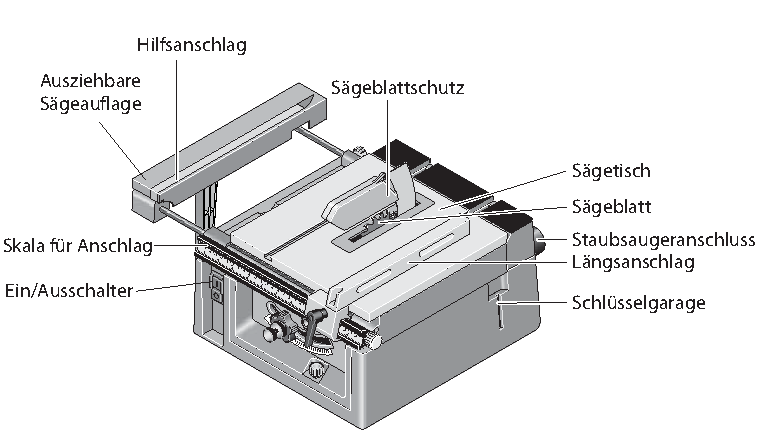
\includegraphics[width=0.8\textwidth]{bilder/saege-sketch.pdf}
    \caption{Feintischkreissäge FET von Proxxon}
    \label{fig:sketch}
\end{figure}

\section{Bestimmungsgemäße Verwendung}
Die Feintischkreissäge FET von Proxxon ist für feine Schnitte von dünnen Materialien, bis 22mm Dicke, gedacht. Abhängig von den verwendeten Sägeblättern können mit der Maschine alle Holzarten, viele NE-Metalle, Keramik und Kunststoffe und Epoxid-Leiterplatten bearbeitet werden. Die entsprechenden Sägeblätter finden später noch eine ausführlichere Erwähnung. Es ist wichtig, die folgenden Anweisungen genau zu beachten, damit die Teischkreissäge nicht zu Gesundheitsschäden führt oder beschädigt wird.\\
Bei der Verwendung der Maschine sollte möglichst der Festool-Staubsauger verwendet werden, da sonst sehr viel Staub und Dreck entsteht. Insbesondere bei Arbeiten mit GFK-Platten (Leiterplatten) muss unbedingt die Absaugung angeschlossen sein. Dabei ist zu beachten, dass die Tischkreissäge an der Steckdose des Saugers mit dem am Staubsauger hängenden Festtool Stromkabel angeschlossen wird und der Sauger auf \enquote{AUTO} steht. Bei Holz kann sich der Einlass der Absaugung (4) an der Oberfräse durch Holzsplitter zusetzen. Bei geringem Absaugeffekt ist die Arbeit zu unterbrechen und die Problemstelle zu finden.\\
Das Werkstück beim Sägen auf die Arbeitsplatte drücken; gefühlvoll und mit wenig Kraft führen; mehr Druck auf die Arbeitsplatte, wenig Druck gegen das Sägeblatt. Führen Sie das Werkstück langsam in das Sägeblatt, besonders wenn das Blatt sehr dünn und die Zähne sehr fein sind, bzw. das Werkstück sehr dick ist.
\textbf{WICHTIG: Die Tischkreissäge darf ausschließlich von eingewiesene Personen verwendet werden.}


\section{Inbetriebnahme}
Maschine vor dem Anschließen und entfernen des Stromkabels stets ausschalten! Dazu Ein-/Ausschalter (19) drücken.

\subsection{Aufstellend der Maschine}
Die Säge muss, um sicheren Betrieb zu gewährleisten, auf einer standfesten Platte, in unserem Fall der Werkbank, befestigt werden. Dabei wird die Tischkreissäge mit dem Untergrund über Spannzangen, befinden sich in Schublade W4, arretiert. \\ \\
\textbf{Merke:}
Sicheres und exaktes Arbeiten ist nur mit einer sorgfältigen Befestigung möglich!

\subsection{Sägeblattschutz}

Die Tischkreissäge ist mit einem Sägeblattschutz ausgerüstet. Diese ist so konzipiert, dass er automatisch so weit wie beim Sägen erforderlich nach oben fährt und anschliessend wie-
der in seine Ruheposition zurückfällt. Er passt sich außerdem an verschieden eingestellte Schnittiefen an.

\textbf{Achtung:} 
Der Sägeblattschutz ist ein wichtiges Sicherheitsutensil und darf auf gar keinen Fall irgendwie manipuliert oder demontiert werden. Der Betrieb der Säge ohne diesen Schutz ist untersagt.
Beim Aufstellen und Transport der Säge immer darauf achten, dass die obere Sägeblattabdeckung sich in Ihrer richtigen Position befindet. Von den freiliegenden spitzen Zähnen des Sägeblattes geht eine erhebliche Verletzungsgefahr aus!


\section{Einstellungen}
\subsection{Höhenverstellung des Sägeblattes}

Zur Anpassung der Schnitttiefe sollte die Position des Sägeblattes in der Höhe reguliert werden. Dies optimiert auf der einen Seite die Sägeleistung, des weiteren wird durch die Begrenzung des freilaufenden Sägeblattanteils die Verletzungsgefahr reduziert.

\begin{figure} 
	\centering
	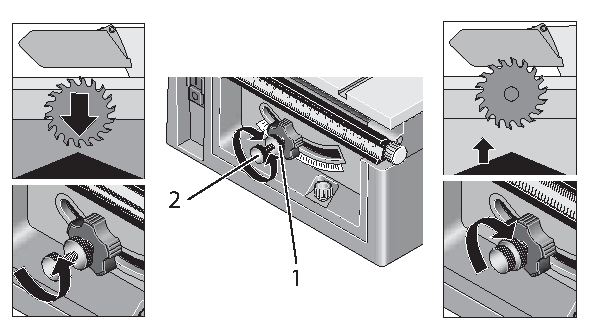
\includegraphics[width=0.6\textwidth]{bilder/saegeverstellung.pdf}
	\caption{Höhenverstellung des Sägeblattes}
	\label{fig:verstellung}
\end{figure}


\textbf{Anleitung:} \\
\renewcommand{\labelenumi}{\alph{enumi})}
\begin{enumerate}
	\item Die größere Verstellschraube 1 (Abbildung \ref{fig:verstellung}) an der vorderen Bedienfläche lösen und aufdrehen
	\item An der kleineren Verstellschraube 2 wird die Sägeblattposition eingestellt: Drehen im Uhrzeigersinn verstellt das Blatt nach oben, drehen gegen den Uhrzeigersinn nach unten.
	\item Nach Erreichen der gewünschten Position die Verstellschraube 1 festdrehen.
\end{enumerate}


\subsection{Verstellen der Sägeblattneigung}

Für Gehrungsschnitte kann das Sägeblatt geneigt werden. Mit Hilfe der Winkelskala wird die gewünschte Neigung eingestellt, bzw. kann abgelesen werden.

\textbf{Anleitung:} \\
\renewcommand{\labelenumi}{\alph{enumi})}
\begin{enumerate}
	\item Verstellrad 1 (Abbildung \ref{fig:winkelverstellung}) lösen.
	\item Sägeblatt mit dem Verstellrad nach rechts schwenken.
	\item Gewünschten Winkel mit dem Zeiger 2 an der Winkelskala 3 einstellen, bzw. ablesen.
	\item Sägeblattstellung durch Zudrehen der Verstellschraube 1 arretieren.
\end{enumerate}

\begin{figure} [h]
	\centering
	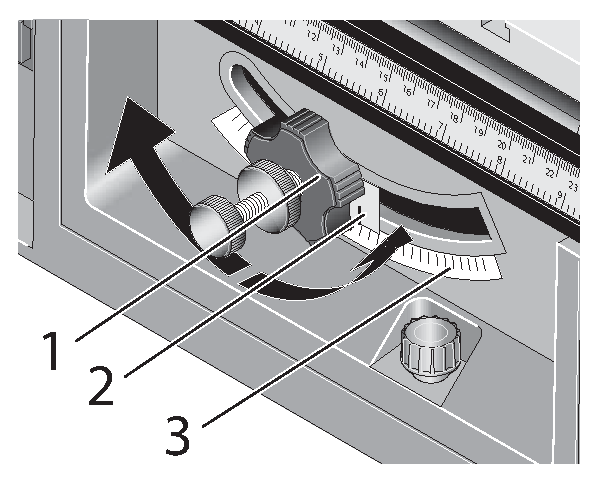
\includegraphics[width=0.6\textwidth]{bilder/winkelverstellung.pdf}
	\caption{Verstellung der Sägeblattneigung}
	\label{fig:winkelverstellung}
\end{figure}

\subsubsection{Ausziehen des Sägetisches}

In einigen Fällen reicht die vorhandene Auflegeläche nicht aus, um größere Werkstücke bearbeiten zu können. Der Sägetisch ist bei diesem Gerät ausziehbar konstruiert, um größere Werkstücke sicher aufliegen zu lassen und diese dann bearbeiten zu können. 


\textbf{Anleitung:} \\
\renewcommand{\labelenumi}{\alph{enumi})}
\begin{enumerate}
	\item Die gelbfarbene Anschlagkante, siehe Abbildung 1 (22), entfernen.
	\item Anschließend den Sägetisch in die gewünschte Postion nach außen ziehen. Mit dem vorhandenen Schwenkhebel abstützen.
	\item Mit einer kleinen Verstellschraube kann der ausziehbare Sägetisch in der gewünschten Position festgeklemmt werden.
	\item Die Anschlagkante wieder in ihre Ursprungsposition drücken, so dass eine plane Oberfläche entsteht. Nun kann mit der Säge gearbeitet werden.
\end{enumerate}

\subsection{Sägeblatt  wählen}
Bevor mit der Arbeit begonnen werden kann, muss das geeignete Sägeblatt gewählt werden. Zu berücksichtigen dabei sind so unterschiedliche Eigenschaften wie Werkstückmaterial, Beanspruchung und die gewünschte Schnittqualität. Dafür gibt es vier verschiedene Sägeblätter, mit denen die Maschine betrieben werden kann:

\begin{table}[h]
	\centering
	\begin{tabular}{lll}
		&\textbf{Sägeblatt}  & \textbf{Materialien} \\
		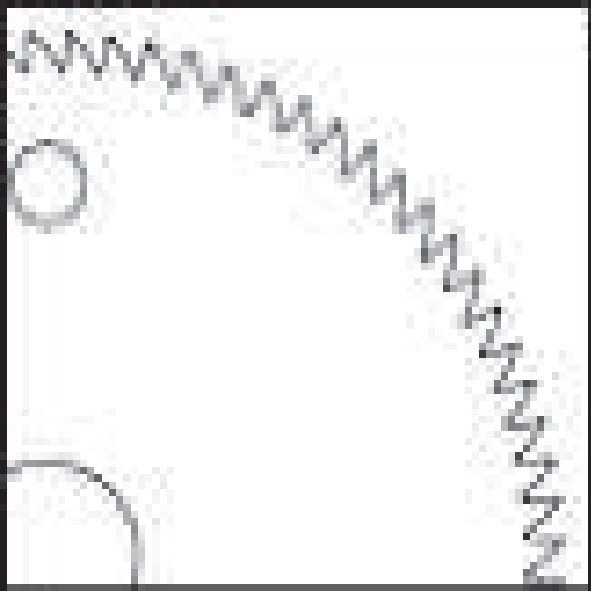
\includegraphics[width=1cm]{bilder/super_cut.pdf}&Super-Cut & Für weichere Hölzer und Kunststoffe \\
		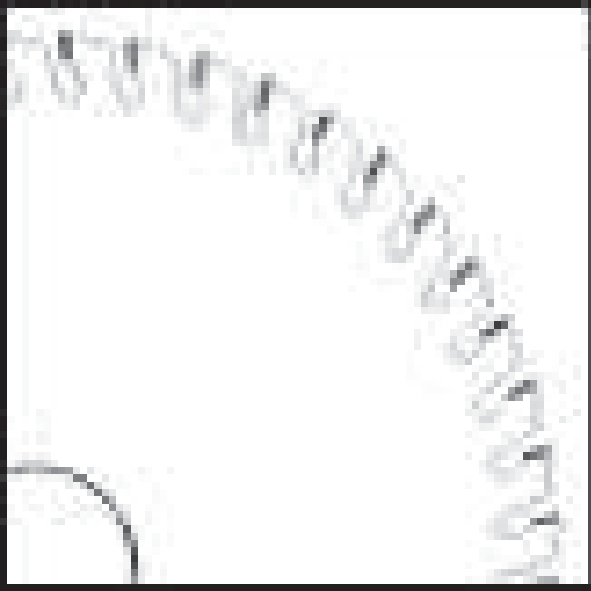
\includegraphics[width=1cm]{bilder/36zahne.pdf}&36 Zähne, Hartmetall &  Balsaholz, Sperrholz, Weichholz, Hartholz, Kunststoff und Aluminium\\
		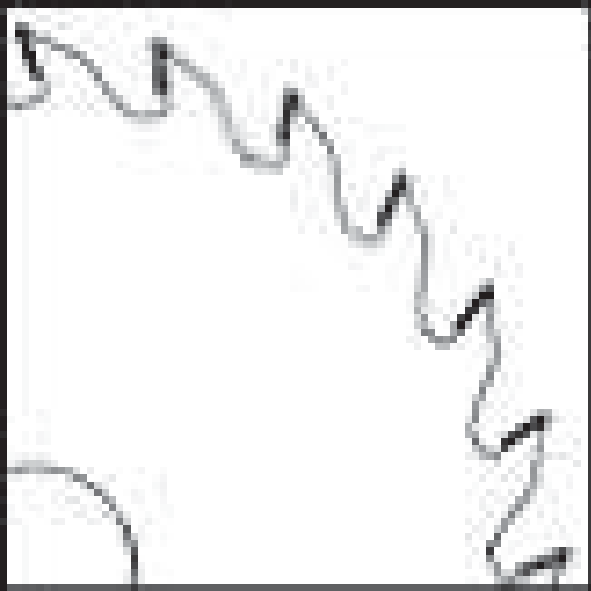
\includegraphics[width=1cm]{bilder/24zahne.pdf}&24 Zähne, Hartmetall & Aluminium, Hartholz, Spanplatten, Kunststoff \\
		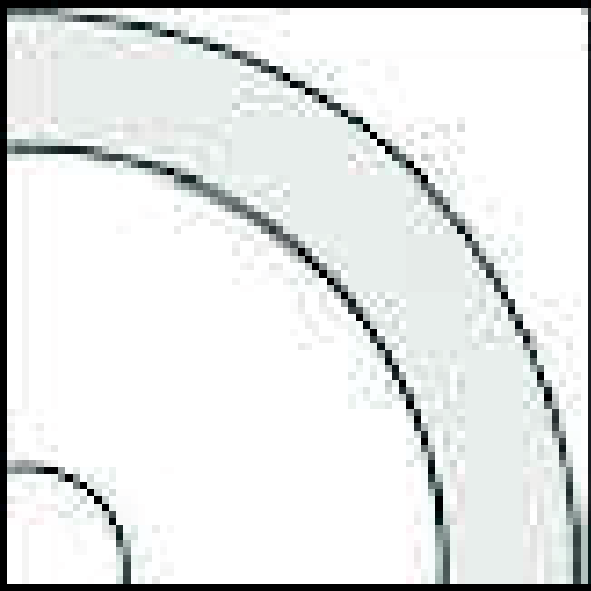
\includegraphics[width=1cm]{bilder/diamant.pdf}&Diamantblatt & Speziell zum Schneiden von keramischen Teilen und GFK-Platten
	\end{tabular}
\end{table}

\subsection{Wechsel des Sägeblattes}

Nachdem die Wahl des Sägeblattes für das zu schneidende Werkstück getroffen ist, ist es notwendig dieses ggf. in der Säge zu tauschen. Hierzu bitte einen Betreuer zur Beihilfe bitten, da hierbei ein großes Gefahrenpotential besteht. 


\textbf{Anleitung:} \\
\renewcommand{\labelenumi}{\alph{enumi})}
\begin{enumerate}
	\item \textbf{Netzstecker ziehen!}
	\item Sägeblatt wie in Kapitel „Höhenverstellung des Sägeblattes“ beschrieben nach unten drehen.
	\item Das Gehäuse nun aufklappen.
	\item Zum Loslösen der Schraube  muss die Welle, auf der das Sägeblatt montiert ist, blockiert werden. Dazu wird ein kleiner Innensechskantschlüssel in eine Bohrung auf dem Sägetisch eingeführt und von dort durch eine Querbohrung in der Sägeblattwelle gesteckt. Gegebenfalls muss diese Bohrung durch Drehen des Sägeblattes von Hand etwas „gesucht“ werden.
	\item Mit einem größeren Innensechskantschlüssel die Zylinderkopfschraube lösen, herausdrehen und zusammen mit dem Sägeblatt entnehmen.
	\textbf{Achtung:}
	Die Zähne der Sägeblätter sind auch bei verschlissenen Sägeblättern noch sehr scharf! Verletzungsgefahr!
	\item Altes Sägeblatt nach oben entnehmen und durch die Sägeblattöffnung und das neue Sägeblatt auf die Welle aufsetzen. Auf richtigen Sitz der Sägeblattbohrung am Wellenbund achten!
	\item Sägeblatt mit der Zylinderkopfschraube wieder eindrehen und anziehen. Beachten, dass die Sägewelle weiterhin mit dem kleinen Innensechskantschlüssel blockiert bleiben muss.
	\item Arretierung lösen, Geräteoberteil wieder nach unten klappen und mit der Verstellschraube verriegeln.
\end{enumerate}

\section{Arbeiten mit einer Tischkreissäge}

\subsection{Längsanschläge}
Längsanschläge sind ein unentbehrliches Hilfsmittel, um Werkstücke exakt sägen zu können. Das Werkstück wird einfach beim Sägevorgang am Längsanschlag mit leichtem Druck entlang geführt, somit entspricht das Maß des fertig gesägten Werkstückes dem des Abstands von Sägeblatt zur Anschlagkante des Längsanschlages. \\
Zur Einstellung des Längsanschlags lässt sich, falls gewünscht, die Skala an der Gehäusevorderseite heranziehen.

\subsubsection{Einsetzen und Entnehmen}
Der Längsanschlag wird seitlich (von rechts oder links) in die Führungen auf dem Sägetisch eingesetzt. Bitte stellen Sie beim Verschieben, Einsetzen bzw. Entnehmen des Längsanschlags sicher, dass beide Feststellmöglichkeiten gelöst sind! Bei dem Betrieb der Säge sind die Anschläge fest zu arretieren. 

\subsubsection{Einstellen des Längsanschlags}

Das grobe Einstellen durch einfaches Verschieben des Längsanschlags ohne Zuhilfenahme der oberen Skala ist für die meisten Fälle ausreichend.\\
\textbf{Achtung!}Stellen Sie sicher, dass bei allen Einstellarbeiten der Netzstecker gezogen ist! \\

\textbf{Anleitung:} \\
\renewcommand{\labelenumi}{\alph{enumi})}
\begin{enumerate}
	\item Bitte zum Verschieben des Anschlags die Fixierschrauben des Längsanschlages lösen.
	\item Der Längsanschlag unter Zuhilfenahme der Skala auf der Oberseite in seiner Führung verschieben. 
	\item Durch Festziehen der Fixierschrauben Längsanschlag arretieren.
	
\end{enumerate}

\subsection{Hilfsanschlag}
Damit größere Werkstücke problemlos zugeschnitten werden können, kann mit dem Hilfsanschlag gearbeitet werden. Dazu muss zunächst der Sägetisch ausgezogen werden in dem Kapitel „Auszeihen des Sägetisches“ beschrieben. Anschließend wird die Anschlagkante nicht „versenkt“, sondern bleibt einfach außen. \\
Die Entfernung zum Sägeblatt bestimmt die Sägebreite, diese kann variiert werden. Zum Sägen den Anschlag immer durch Anziehen der Fixierschraube festziehen.
\subsection{Winkelanschlag}

Wird ein winkelig zugeschnittenes Werkstück oder ein Gehrungsschnitt benötigt, kann dies mit Hilfe eines Winkelanschlags erfolgen. Dieser läuft in den dafür vorgesehenen Führungen entweder rechts oder links vom Sägeblatt entlang, wie benötigt.

\begin{figure} [h]
	\centering
	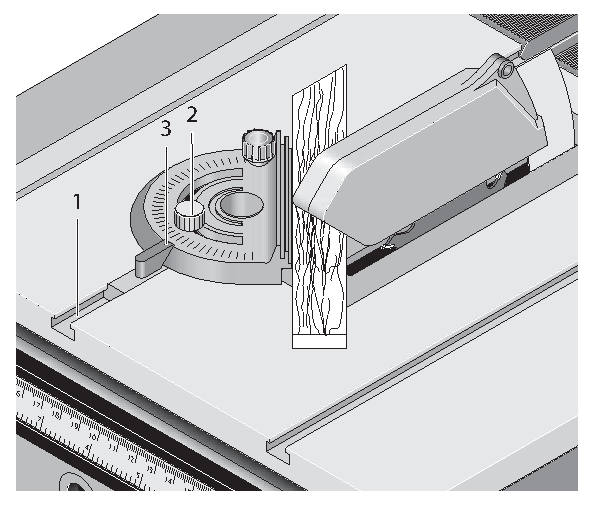
\includegraphics[width=0.6\textwidth]{bilder/Winkelanschlag.pdf}
	\caption{Verwendung des Winkelanschlages}
	\label{fig:winkelanschlag}
\end{figure}

\textbf{Anleitung:} \\
\renewcommand{\labelenumi}{\alph{enumi})}
\begin{enumerate}
	\item Winkelanschlag in die Führung 1 rechts oder links vom Sägeblatt einsetzen, wie in Abbildung \ref{fig:winkelanschlag} zu sehen.
	\item Verstellschraube 2 lösen, den gewünschten Winkel an der Skala 3 einstellen und die Verstellschraube wieder festziehen.

\end{enumerate}


%\newpage
\section{Quellen und Rechte}
\label{quellen}
Alle Rechte an Grafiken, Tabellen und Textabschnitte, welche aus der Proxxon Originalbetriebsanleitung übernommen wurden liegen bei Proxxon. Die \glqq Originalbetriebsanleitung\grqq liegt der Maschine bei und ist online auf \url{www.proxxon.de} zu finden. Proxxon hat dieses Dokument weder gelesen, noch auf Vollständigkeit oder Richtigkeit geprüft und übernimmt keine Haftung.

\end{document}
